\documentclass{beamer}
\usepackage{amsmath}
\usepackage{amssymb}
\usepackage{xparse}
\usepackage{gvv}
\usetheme{Madrid}
\usecolortheme{default}
\usepackage{tfrupee}

\title{\textbf{5.8.3}}
\author{\textbf{Aditya Mishra-EE25BTECH11005}}
\date{October 10, 2025}

\begin{document}

\begin{frame}
\titlepage
\end{frame}

\begin{frame}{Question}
5 pencils and 7 pens together cost \rupee50, whereas 7 pencils and 5 pens together cost \rupee46.  
Find the cost of one pencil and that of one pen.
\end{frame}

\begin{frame}{Solution}
\textbf{Converting to Equations:}\\[4pt]
Let the cost of one pencil be \(x\), pen be \(y\).
\begin{align}
5x + 7y &= 50 \\
7x + 5y &= 46
\end{align}
\end{frame}

\begin{frame}{Solution}
\textbf{Forming Augmented Matrix:}
\begin{align}
\augvec{2}{1}{5 & 7 & 50 \\ 7 & 5 & 46}
\end{align}
\end{frame}

\begin{frame}{Solution}
\textbf{Row Operation and Reduction:}\\
\begin{align}
\augvec{2}{1}{5 & 7 & 50 \\ 7 & 5 & 46}
&\xrightarrow{\,R_2 \rightarrow R_2 - \frac{7}{5} R_1\,}
\augvec{2}{1}{5 & 7 & 50 \\ 0 & -4.8 & -24}
\end{align}
\end{frame}

\begin{frame}{Solution}
\textbf{Back Substitution:}
\begin{align}
-4.8y &= -24 \implies y = 5 \\
5x + 7y &= 50 \implies 5x + 35 = 50 \implies x = 3
\end{align}
\end{frame}

\begin{frame}{Solution}
\textbf{Final Solution:}
\begin{align}
\vec{x} = \myvec{3 \\ 5}
\end{align}
Cost of one pencil is \rupee3 and one pen is \rupee5.
\end{frame}

\begin{frame}{Plot}
\begin{figure}
    \centering
    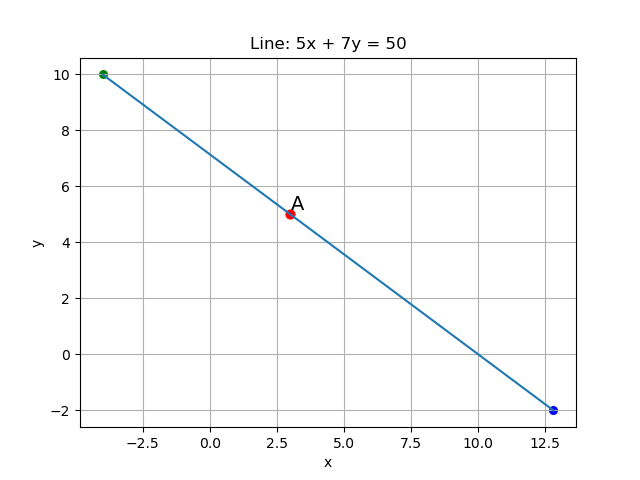
\includegraphics[width=0.8\columnwidth]{Figs/Figure_1.png}
\end{figure}
\end{frame}

\begin{frame}{Codes}
\centering
For Codes, refer to the URL below:  
\url{https://github.com/Aditya-Mishra11005/ee1030-2025/tree/main/ee25btech11005/matgeo/5.8.3/Codes}
\end{frame}

\end{document}

